\documentclass[aspectratio=169]{beamer}

% Lines related with beamer theme
\usetheme[progressbar=frametitle]{metropolis}
%\setbeamertemplate{frame numbering}[fraction]

\setbeamertemplate{caption}{\raggedright\insertcaption\par}


% Lines related with latex packages
\usepackage{amsmath,amsfonts,amssymb}
\usepackage{mathtools} 
\usepackage{multicol}
\usepackage{tikz}
\usetikzlibrary{arrows.meta,positioning,fit}
\usepackage{xcolor}
\usepackage{bm}
\usepackage{adjustbox}


% First slide info
\author{Antón de la Fuente Suárez-Pumariega}
\title{Decentralized decision power and information sharing in horizontal logistics collaboration}
\institute{
\includegraphics[scale=0.08]{maastricht-logo}}
\date{18th of August, 2021}
\def\titlepage{
  \usebeamertemplate{title page}
}

\begin{document}

% I few lines selecting some parameters of the beamer theme
\metroset{block=fill}
\metroset{sectionpage=simple}
\metroset{subsectionpage=simple}

%Tittle slide
\maketitle

%Table of contents
\begin{frame}{Agenda}
\setbeamertemplate{section in toc}[sections numbered]
\setbeamertemplate{subsection in toc}[subsections numbered]
	\tableofcontents
\end{frame}

%\metroset{sectionpage=none}
\section{Introduction}

\begin{frame}{Horizontal logistics collaboration}

\begin{itemize}
\setlength\itemsep{1em}
\item Central planning
\item Decentralized systems $\begin{cases}
\text{Auction-based}\\[5pt]
\text{\only<2>{\color{blue}}Non auction-based}
\end{cases}$
\end{itemize}

\usetikzlibrary{arrows.meta,positioning}
\end{frame}

\section{The network design - multicommodity flow problem}

\begin{frame}{\secname}

\begin{columns}

\begin{column}{0.5\textwidth}
\textbf{Commodities:}
\begin{table}
\begin{tabular}{ccccc}
& $o(k)$ & $t(k)$ & $d_k$ & $r_k$ \\\hline
$\color{red}k^1$ & 1 & 2 & 1 & 10 \\
$\color{red}k^2$ & 1 & 4 & 1 & 10 \\
$\color{red}k^3$ & 3 & 1 & 1 & 10 
\end{tabular}
\end{table}
\bigskip

\textbf{Edges:}
\begin{table}
\begin{tabular}{ccc}
& $q_e$ & $c_e$ \\\hline
$\forall e \in E$ & 2 & 5 \\
\end{tabular}
\end{table}
\end{column}

\begin{column}{0.5\textwidth}
\only<1>{
\begin{figure}
	\centering	
	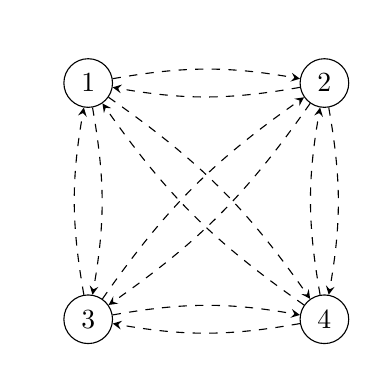
\begin{tikzpicture}
	\begin{scope}[every node/.style={circle,draw,align=center,text width = 5pt}]
		\node (1) at (0,0) {1};
		\node (2) at (3,0) {2};
		\node (3) at (0,-3) {3};
		\node (4) at (3,-3) {4};
	\end{scope}
	\begin{scope}[every edge/.style={dashed,draw,bend left=10}]
		\draw[-stealth] (1) edge node[above] {\phantom{$k^1$}} (2);
		\draw[-stealth] (2) edge (1);
		\draw[-stealth] (1) edge (3);
		\draw[-stealth] (3) edge node[left] {\phantom{$k^3$}} (1);
		\draw[-stealth] (1) edge node[right=9pt] {\phantom{$k^2$}} (4);
		\draw[-stealth] (4) edge (1);
		\draw[-stealth] (2) edge (3);
		\draw[-stealth] (3) edge (2);
		\draw[-stealth] (2) edge (4);
		\draw[-stealth] (4) edge (2);
		\draw[-stealth] (3) edge (4);
		\draw[-stealth] (4) edge (3);
	\end{scope}
	\end{tikzpicture}
	\caption{Original network.}
	\end{figure}
}

\only<2>{
\begin{figure}
	\centering	
	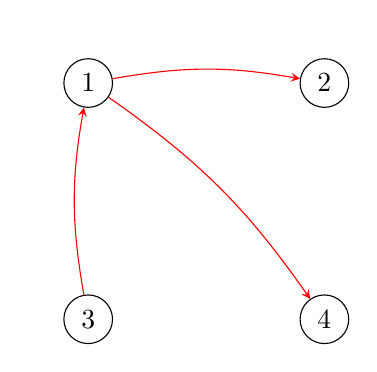
\begin{tikzpicture}
	\begin{scope}[every node/.style={circle,draw,align=center,text width = 5pt}]
		\node (1) at (0,0) {1};
		\node (2) at (3,0) {2};
		\node (3) at (0,-3) {3};
		\node (4) at (3,-3) {4};
	\end{scope}
	\begin{scope}[every edge/.style={draw,bend left=10}]
		\draw[-stealth,red] (1) edge node[above] {\phantom{$k^1$}}(2);
	
		\draw[-stealth,red] (3) edge node[left] {\phantom{$k^3$}} (1);
		\draw[-stealth,red] (1) edge node[right=9pt] {\phantom{$k^2$}} (4);
	
	\end{scope}Example
	\end{tikzpicture}
	\caption{Design of the network.}
	\end{figure}
}

\only<3>{
\begin{figure}
	\centering	
	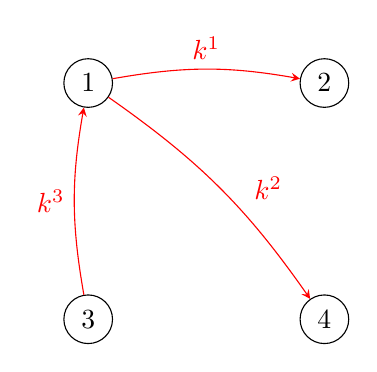
\begin{tikzpicture}
	\begin{scope}[every node/.style={circle,draw,align=center,text width = 5pt}]
		\node (1) at (0,0) {1};
		\node (2) at (3,0) {2};
		\node (3) at (0,-3) {3};
		\node (4) at (3,-3) {4};
	\end{scope}
	\begin{scope}[every edge/.style={draw,bend left=10}]
		\draw[-stealth,red] (1) edge node[above] {$k^1$} (2);
		\draw[-stealth,red] (3) edge node[left] {$k^3$} (1);
		\draw[-stealth,red] (1) edge node[right=9pt] {$k^2$} (4);
		
	\end{scope}
	\end{tikzpicture}
	\caption{Route the commodities.}
	\end{figure}
}
\end{column}

\end{columns}
\end{frame}

\begin{frame}{\secname: ILP}

\begin{itemize}
\item We model the problem as an ILP, $\quad \pmb{P_i}\ \forall i \in N$.

\begin{align}
        &  P_i: \quad \max  &  \sum_{k\in \Theta^i} \sum_{e \in \delta^+(t(k))\cap E^i} f_e^k \cdot d_k \cdot r_k - \sum_{e\in E^i} u_e\cdot c_e \hspace{20pt} &&
	\end{align}
	
\item Subject to different constraints
\end{itemize}
	

    
\end{frame}

\begin{frame}{\secname}

\begin{columns}

\begin{column}{0.5\textwidth}
\textbf{Commodities:}
\begin{table}
\begin{tabular}{ccccc}
& $o(k)$ & $t(k)$ & $d_k$ & $r_k$ \\\hline
$\color{red}k^1$ & 1 & 2 & 1 & 10 \\
$\color{red}k^2$ & 1 & 4 & 1 & 10 \\
$\color{red}k^3$ & 3 & 1 & 1 & 10 \\
$\color{blue}k^4$ & 2 & 4 & 1 & 10
\end{tabular}
\end{table}
\bigskip

\textbf{Edges:}
\begin{table}
\begin{tabular}{ccc}
& $q_e$ & $c_e$ \\\hline
$\forall e \in E$ & 2 & 5 \\
\end{tabular}
\end{table}
\end{column}

\begin{column}{0.5\textwidth}
\only<1>{
\begin{figure}
	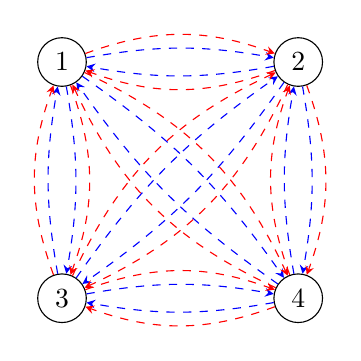
\begin{tikzpicture}
	\centering	
	\begin{scope}[every node/.style={circle,draw,align=center,text width = 5pt}]
		\node (1) at (0,0) {1};
		\node (2) at (3,0) {2};
		\node (3) at (0,-3) {3};
		\node (4) at (3,-3) {4};
	\end{scope}
	\begin{scope}[every edge/.style={dashed,draw,bend left=10},blue]
		\draw[-stealth] (1) edge (2);
		\draw[-stealth] (2) edge (1);
		\draw[-stealth] (1) edge (3);
		\draw[-stealth] (3) edge (1);
		\draw[-stealth] (1) edge (4);
		\draw[-stealth] (4) edge (1);
		\draw[-stealth] (2) edge (3);
		\draw[-stealth] (3) edge (2);
		\draw[-stealth] (2) edge (4);
		\draw[-stealth] (4) edge (2);
		\draw[-stealth] (3) edge (4);
		\draw[-stealth] (4) edge (3);
		
	\end{scope}
	\begin{scope}[every edge/.style={dashed,draw,bend left=20},red]
		\draw[-stealth] (1) edge (2);
		\draw[-stealth] (2) edge (1);
		\draw[-stealth] (1) edge (3);
		\draw[-stealth] (3) edge (1);
		\draw[-stealth] (1) edge (4);
		\draw[-stealth] (4) edge (1);
		\draw[-stealth] (2) edge (3);
		\draw[-stealth] (3) edge (2);
		\draw[-stealth] (2) edge (4);
		\draw[-stealth] (4) edge (2);
		\draw[-stealth] (3) edge (4);
		\draw[-stealth] (4) edge (3);
	\end{scope}
	\end{tikzpicture}
	\caption{Original network.}
	\end{figure}
}

\only<2>{
\begin{figure}
	\centering	
	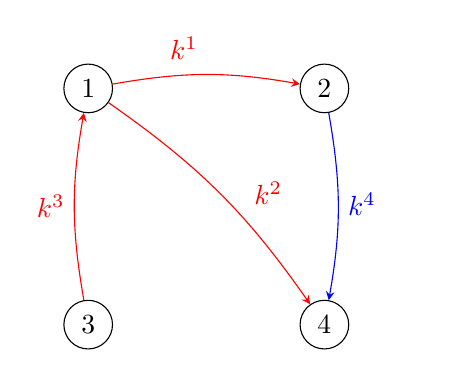
\begin{tikzpicture}
	\begin{scope}[every node/.style={circle,draw,align=center,text width = 5pt}]
		\node (1) at (0,0) {1};
		\node (2) at (3,0) {2};
		\node (3) at (0,-3) {3};
		\node (4) at (3,-3) {4};
	\end{scope}
	\begin{scope}[every edge/.style={draw,bend left=10}]
		\draw[-stealth,red] (1) edge node[above] {$k^1$\phantom{, $\color{red}k^2$}}(2);
		\draw[-stealth,red] (3) edge node[left] {$k^3$} (1);
		\draw[-stealth,red] (1) edge node[right=9pt] {$k^2$} (4);
		\draw[-stealth,blue,bend left=20] (2) edge  node[right] {$k^4$\phantom{, $\color{red}k^2$}} (4);
	\end{scope}
	\end{tikzpicture}
	\caption{Solution without cooperation.}
	\end{figure}
}

\only<3>{
\begin{figure}
	\centering	
	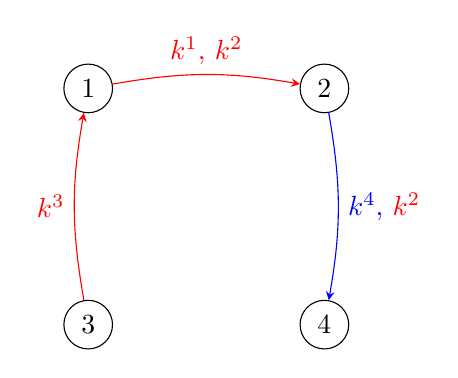
\begin{tikzpicture}
	\begin{scope}[every node/.style={circle,draw,align=center,text width = 5pt}]
		\node (1) at (0,0) {1};
		\node (2) at (3,0) {2};
		\node (3) at (0,-3) {3};
		\node (4) at (3,-3) {4};
	\end{scope}
	\begin{scope}[every edge/.style={draw,bend left=10}]
		\draw[-stealth,red] (1) edge node[above] {$k^1$, $k^2$}(2);
		\draw[-stealth,red] (3) edge node[left] {$k^3$} (1);
		\draw[-stealth,blue,bend left=20] (2) edge  node[right] {$k^4$, $\color{red}k^2$} (4);
	\end{scope}
	\end{tikzpicture}
	\caption{Cooperative solution.}
	\end{figure}
}
\end{column}

\end{columns}
\end{frame}

\section{Allocation rule}

\begin{frame}{\secname}
\begin{enumerate}
	\setlength\itemsep{1em}
    \item The revenues generated by any served commodity are
    allocated to its owner.
    \item The activation cost of any active edge is paid by its owner.
    \item The price of using an unit of capacity on an edge $e\in E$ owned by agent $w(e)$ for any other member of the coalition, $i\in N\setminus\{w(e)\}$, is equal to $\dfrac{c_e}{q_e}$.
\end{enumerate}
\end{frame}


\section{Three systems with central authority}
\begin{frame}{\secname}
\begin{itemize}
\setlength\itemsep{1em}

\item A central authority with certain decision power.
\item Agents have to share certain amount of information to cooperate.
\item 3 systems: $\begin{cases}
\text{Fully centralized cooperation system (FCCS),}\\
\text{Partial cooperation system (PCS),} \\
\text{Residual cooperation system (RCS).}
\end{cases}$
\end{itemize}
\end{frame}

\subsection{Fully centralized cooperative system (FCCS)} 
\begin{frame}{\subsecname}
\begin{itemize}
\setlength\itemsep{1em}
\item A central planning system $\Longrightarrow$ Central authority with \textcolor{blue}{full information} and \textcolor{blue}{all the decision power.}
\item Commodities and edges of all the agents are aggregated into a single bigger problem.
\item Final profit allocation must be \textcolor{red}{individually rational}.
\end{itemize}
\end{frame}

\subsection{Partial cooperative system (PCS)}

%\begin{frame}{\subsecname}
%Agents solve the network design - problem in two stages:
%\begin{enumerate}
%	\setlength\itemsep{1em}
%	\item Agents decide which edges to activate
%	\item The central authority routes the commodities %through the active edges
%\end{enumerate}
%\end{frame}

\begin{frame}{\subsecname}

\begin{figure}[ht!]
\centering
\begin{adjustbox}{width=\textwidth, totalheight=\textheight-2\baselineskip,keepaspectratio}
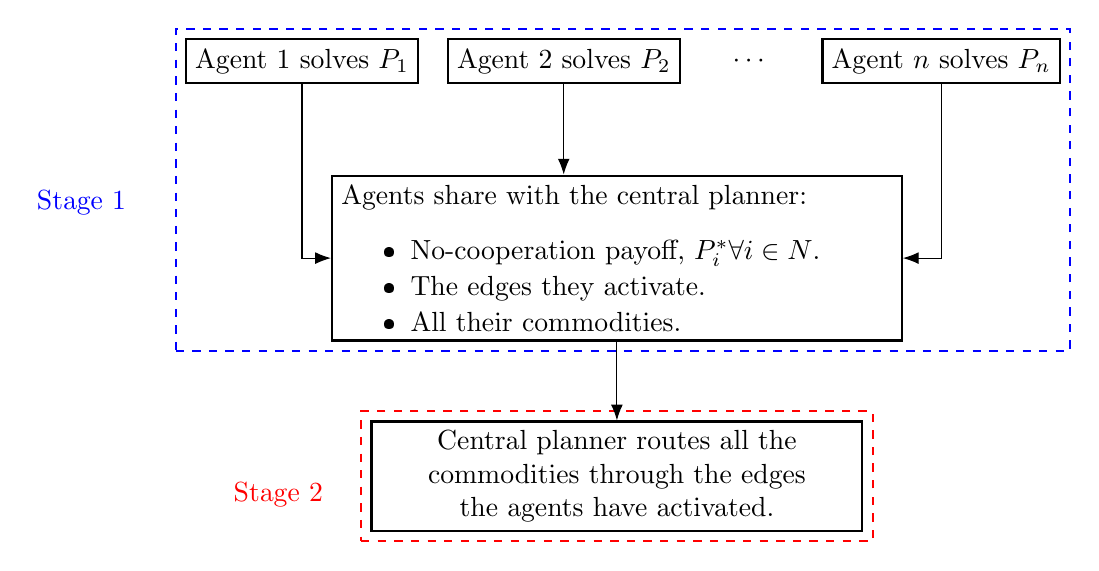
\begin{tikzpicture}
	\begin{scope}[every node/.style={rectangle,draw,thick,minimum height=16pt,minimum width =30pt}]
		\node (A1) at (-4,0) {Agent 1 solves $P_1$};
		\node[right =10pt of A1] (A2) {Agent 2 solves $P_2$};
		\node[draw=none,right =10pt of A2] (pass) {$\cdots$ };
		\node[right =10pt of pass] (An) {Agent $n$ solves $P_n$};
		\node[align = left,text width=7cm] (shares) at (0,-2.5) {Agents share with  the  central planner:
		\begin{itemize}
			\itemsep-3pt 
        		\item No-cooperation payoff, $P^*_i \forall i \in N$.
        		\item The edges they activate.
        		\item All their commodities.
   		 \end{itemize}
    };
    \node[below = of shares,align = center,text width=6cm] (central) {Central planner routes all the commodities through the edges the agents have activated.};
    
    \node [fit=(A1) (An) (shares),draw,dashed,thick,blue] {};
    \node[draw=none,blue] (Stage1) at (-6.8,-1.8) {Stage 1}	;
 	\node [fit=(central) ,draw,dashed,thick,red] {};
 	\node[draw=none,red] (Stage2) at (-4.3,-5.5) {Stage 2}	;
	
	\end{scope}
	
	\begin{scope}
	\draw[-{Latex[length=2mm]}] (A1.south) |- (shares.west);
	\draw[-{Latex[length=2mm]}] (A2) edge (A2.south|-shares.north);
	\draw[-{Latex[length=2mm]}] (An.south) |- (shares.east);
	\draw[-{Latex[length=2mm]}] (shares) edge (central);

	\end{scope}
\end{tikzpicture}
\end{adjustbox}
\end{figure}
\end{frame}

\subsection{Residual cooperation system (RCS)}
\begin{frame}{\subsecname}

\begin{figure}[ht!]
\centering
\begin{adjustbox}{width=\textwidth, totalheight=\textheight-2\baselineskip,keepaspectratio}
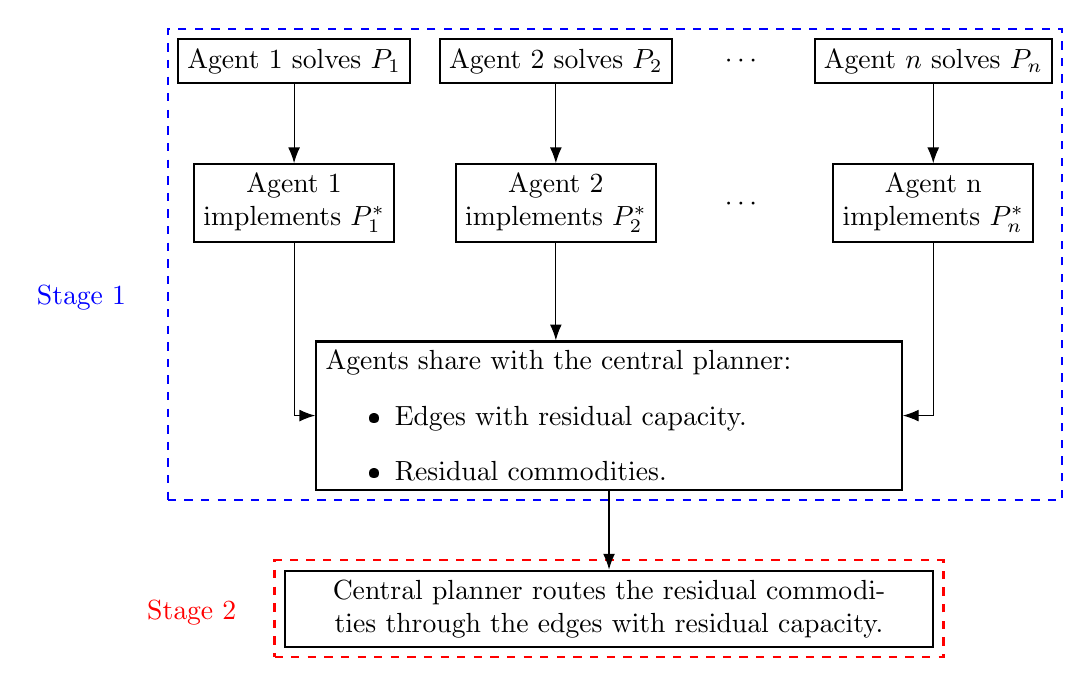
\begin{tikzpicture}
	\begin{scope}[every node/.style={rectangle,draw,thick,minimum height=16pt,minimum width =30pt}]
		\node (A1) at (-4,0) {Agent 1 solves $P_1$};
		\node[right =10pt of A1] (A2) {Agent 2 solves $P_2$};
		\node[draw=none,right =10pt of A2] (pass) {$\cdots$ };
		\node[right =10pt of pass] (An) {Agent $n$ solves $P_n$};
		\node[below = of A1,align = center] (A1impl) {Agent 1 \\ implements $P_1^*$};
		\node[below = of A2,align = center] (A2impl) {Agent 2 \\ implements $P_2^*$};
		\node[draw=none,below =35pt of pass] (pass2) {$\cdots$ };
		\node[below = of An,align = center] (Animpl) {Agent n \\ implements $P_n^*$};
		\node[align = left,text width=7.2cm] (shares) at (0,-4.5){Agents share with  the  central planner:
		\begin{itemize}

        		\item Edges with residual capacity.
        		\item Residual commodities.
   		 \end{itemize}
    };
    \node[below = of shares,align = center,text width=8cm] (central) {Central planner routes the residual commodities through the edges with residual capacity.};
    
	  \node [fit=(A1) (An) (shares),draw,dashed,thick,blue] {};
    \node[draw=none,blue] (Stage1) at (-6.7,-3) {Stage 1}	;
 	\node [fit=(central) ,draw,dashed,thick,red] {};
 	\node[draw=none,red] (Stage2) at (-5.3,-7) {Stage 2}	;    
    
	\end{scope}
	
	\begin{scope}
	\draw[-{Latex[length=2mm]}] (A1) edge (A1impl);
	\draw[-{Latex[length=2mm]}] (A2) edge (A2impl);
	\draw[-{Latex[length=2mm]}] (An) edge (Animpl);
	\draw[-{Latex[length=2mm]}] (A1impl.south) |- (shares.west);
	\draw[-{Latex[length=2mm]}] (A2impl) edge (A2.south|-shares.north);
	\draw[-{Latex[length=2mm]}] (Animpl.south) |- (shares.east);
	\draw[-{Latex[length=2mm]}] (shares) edge (central);

	\end{scope}
\end{tikzpicture}
\end{adjustbox}
\end{figure}
\end{frame}


\section{Fully Decentralized Iterative Cooperative System}

a
\section{Results}

\section{Discussion}

\end{document}